\section{Background}

Our work focuses on multiple aspects of cloud systems namely storage
area networks or SAN's, usage of SSD's in enterprise environments, and
block level caching. We chose DM-Cache as the block level caching
mechanism to evaluate our work on as it is freely available as a part
of the Linux kernel.

\subsection{Storage Area Networks}

Due to the physical limitation of local storage many enterprise
solutions choose to employ Storage Area Networks or SAN's as they are
more commonly referred to in an attempt to centralize storage access
and provide larger storage capabilities. They also provide for
simplification of virtual machine migration and increased data
reliability. While this solves the issue of storage size it increases
request latency and could possibly create bandwidth issues either on
the network or on the storage devices themselves due to the number of
requests from different machines.

\subsection{Enterprise SSD Usage}

Many enterprise cloud solutions employ SSD's where storage latency or
throughput can be bottlenecks for applications. In work by Lee et al.\
they were able to show that using SSD's for enterprise database
applications resulted in performance gains because of throughput
improvement \cite{EnterpriseSSD}. Their work made the case for usage
of SSD's in enterprise environments.

% maybe some works about caching with SSD %

\subsection{DM-Cache}

DM-Cache is a block-level caching mechanism implemented as a module in
the Linux kernel \cite{DM-Cache}. It allows for specification of a
local cache device where recently used blocks can be stored for faster
access time. It supports both write-through and write-back
functionality for handling cached data. Figure~\ref{fig:dm-cache}
shows the architecture of DM-Cache.

\graphicspath{{../Images/}}

\begin{figure}[t]
  \caption{Architecture of DM-Cache}
  \centering 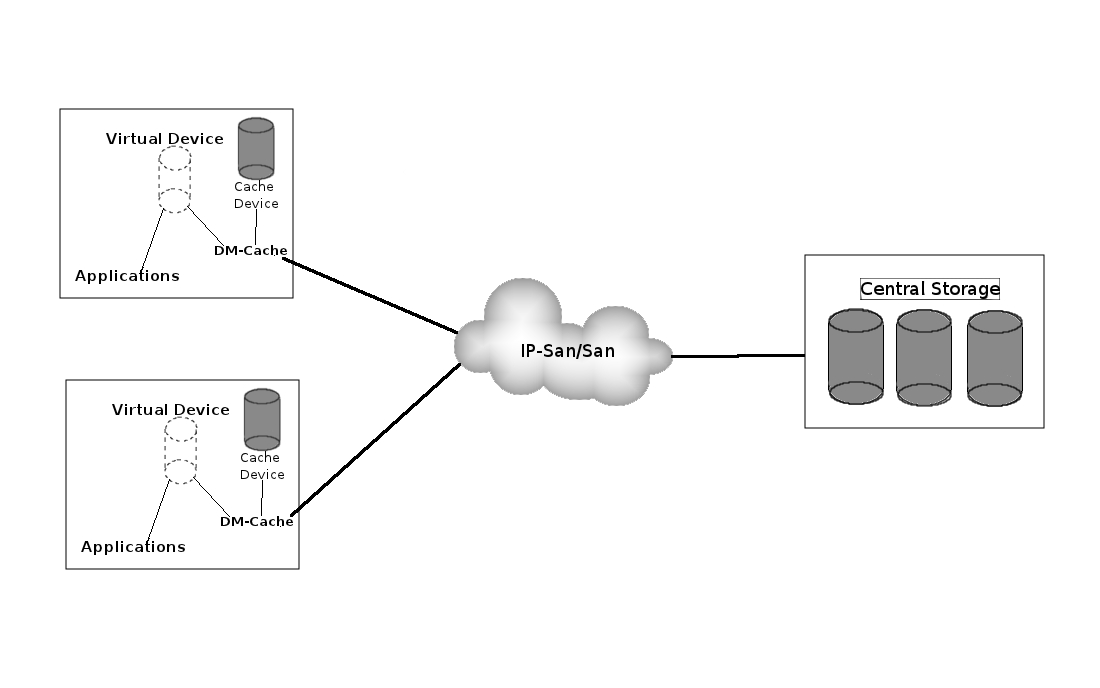
\includegraphics[width=0.5\textwidth]{dm-cache_diagram.jpg}
  \label{fig:dm-cache}
\end{figure}

The purpose of DM-Cache is to cache recently used blocks on local
storage instead of retrieving them from some external storage source
every time they are needed. This helps alleviate network bandwidth as
well as reduce latency and improve response time to requests.

The current metadata persistence scheme in DM-Cache only works if the
cache is properly destroyed. In the event of a failure no metadata is
persisted to disk and the metadata that contains the location of the
cached blocks on the disk is lost.

Another limitation of this scheme is that only blocks that are valid
or have not been modified have their metadata persisted. When a cache
is destroyed all dirty blocks have their changes written back to the
storage device (in the case of a write-back cache) but in the event of
a failure this is not true as blocks can still be pending write back
during this time.
